\begin{margintable}
\scalebox{1.15}{
\begin{tabular}{cc}
	\raisebox{-.05in}{
	\begin{tabular}[b]{r|l} 
	$x$ & $g(x)$ \\ 
	\hline 2.9 & 0.84864 \\ 
	2.99 & 0.86428 \\ 
	2.999 & 0.86585 \\ 
	2.9999 & 0.86601 \\ 
	3.1 & 0.88351 \\ 
	3.01 &  0.86777 \\ 
	3.001 & 0.86620 \\ 
	3.0001 &  0.86604 \\ 
	\end{tabular} } &	
	\raisebox{-.05in}{
	\begin{tabular}[b]{r|l} 
	$x$ & $g(x)$ \\ 
	\hline -0.1 & 0 \\ 
	-0.01 & 0 \\ 
	-0.001 & 0 \\ 
	-0.0001 & 0 \\ 
	0.1 & 0 \\ 
	0.01 & 0 \\ 
	0.001 & 0 \\ 
	0.0001 & 0 \\ 
	\end{tabular} } 
\end{tabular}
} % end scalebox
\caption{Tables for $\ds g(x) = \sin\left(\frac{\pi}{x}\right)$.} \label{T:1-1_Eg2}
\end{margintable}

\begin{marginfigure}
\margingraphics{figures/1_2_Ex1g.eps}
\caption{The graph of \newline $g(x)=\sin\left( \frac{\pi}{x} \right)$ near $3$ and $0$.}\label{fig:1-1_Eg2}
\end{marginfigure}

%	\hspace{0.25in} 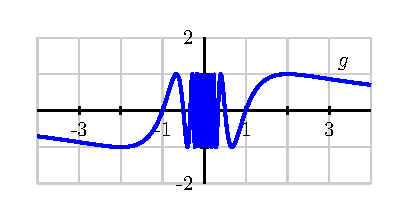
\includegraphics{figures/1_2_Ex1g.eps} 

\begin{example} \label{Ex:1.1.Eg2}
Use both tables and graphical approaches to investigate and, if possible, estimate or determine the value of the limit for the following function at the specified values. 
\[ \ds g(x) = \sin\left( \frac{\pi}{x} \right); \quad a = 3, \ a = 0\]

\solution Again, we construct two tables and a graph, see Table~\ref{T:1-1_Eg2} and Figure~\ref{fig:1-1_Eg2}.

First, as $x \to 3$, it appears from the data (and the graph) that the function is approaching approximately $0.866025$.  To be precise, we have to use the fact that $\frac{\pi}{x} \to \frac{\pi}{3}$, and thus we find that $g(x) = \sin(\frac{\pi}{x}) \to \sin(\frac{\pi}{3})$ as $x \to 3$.  The exact value of $\sin(\frac{\pi}{3})$ is $\frac{\sqrt{3}}{2}$, which is approximately 0.8660254038.  Thus, we see that
$$\lim_{x \to 3} g(x) = \frac{\sqrt{3}}{2}.$$

As $x \to 0$, we observe that $\frac{\pi}{x}$ does not behave in an elementary way.  When $x$ is positive and approaching zero, we are dividing by smaller and smaller positive values, and $\frac{\pi}{x}$ increases without bound.  When $x$ is negative and approaching zero, $\frac{\pi}{x}$ decreases without bound.  In this sense, as we get close to $x = 0$, the inputs to the sine function are growing rapidly, and this leads to wild oscillations in the graph of $g$.  It is an instructive exercise to plot the function $g(x) = \sin\left(\frac{\pi}{x}\right)$ with a graphing utility and then zoom in on $x = 0$.  Doing so shows that the function never settles down to a single value near the origin and suggests that $g$ does not have a limit at $x = 0$.
\end{example}